\subsection{Historia}

Na początku XX wieku, gdy sieci telekomunikacyjne dopiero się rozwijały, wszystkie połączenia zestawiane były ręcznie. W momencie, gdy abonent podnosił słuchawkę telefonu, jego aparat wysyłał sygnał do lokalnej centrali telefonicznej. Na tablicy świetlnej zapalała się lampka informująca telefonistkę o próbie połączenia. Telefonistka odbierała połączenie, pytając, z kim abonent chce się połączyć. Nastpnie wprowadzała odpowiednią wtyczkę do odpowiedniego gniazda na tablicy rozdzielczej, zestawiając fizyczne połączenie między dwoma liniami. Jeśli rozmowa miała się odbyć na większą odległość (np. między miastami) połączenie przekazywane było przez kolejne centrale. Każda centrala po drodze wymagała ręcznej obsługi przez pracujące w nich telefonistki. 

\begin{figure}[!h]
    \centering 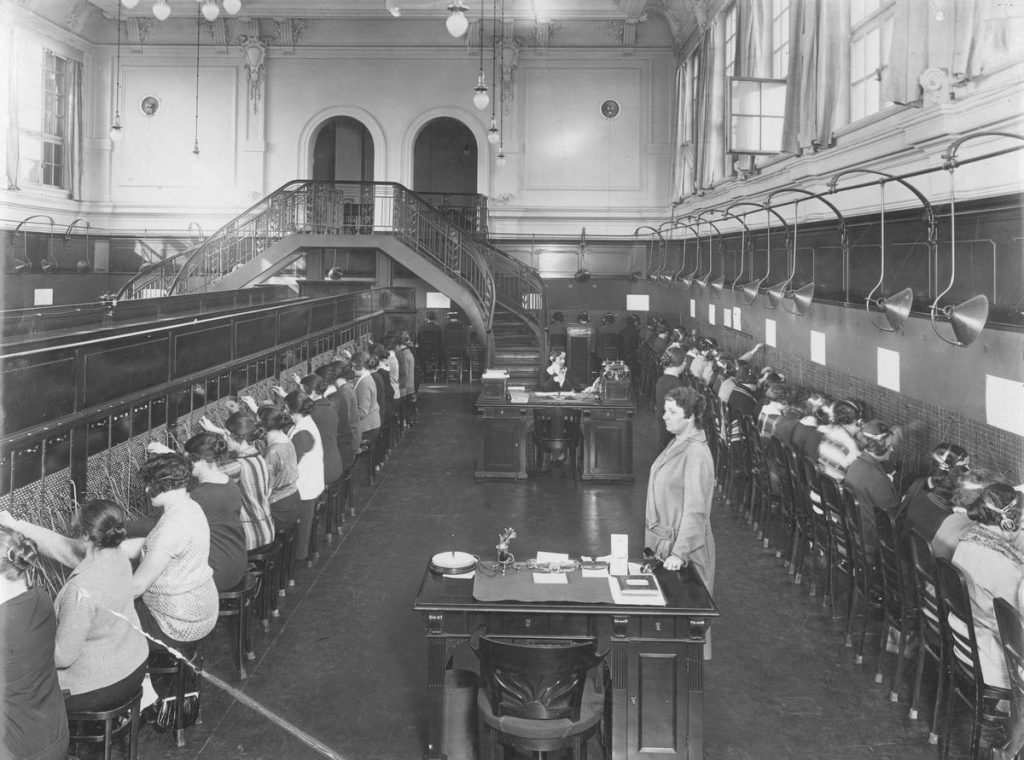
\includegraphics[width=1\linewidth]{telefonistki.jpg}
    \caption{Pracowniczki warszawskiej centrali telefonicznej na zdjęciu z końca lat 20. (domena publiczna).}\label{fig:telefonistki}
\end{figure}

Dziś taki scenariusz wydaje się wręcz absurdalny a oferty pracy dla telefonistek dawno już zniknęły z tablic ogłoszeń. Praca wykonywana przez telefonistki (czyli komutacja łączy) nadal jest potrzebna do prawidłowego funkcjonowania sieci telekomunikacyjnych, lecz wykonywana jest przez programy komputerowe w sposób w pełni zautomatyzowany. Ręczna komutacja była pierwszym krokiem w kierunku rozwoju globalnych sieci telekomunikacyjnych. Choć z dzisiejszej perspektywy wydaje się być bardzo pracochłonna i ograniczająca, bez niej nie powstałyby fundamenty, na których oparto późniejsze systemy automatyczne. Jest to przykład tego, jak technologia stopniowo uwalniała człowieka od bezpośredniej obsługi różnych systemów (dając mu przestrzeń na rózwój w innych obszarach). 

Na zasadzie indukcji możemy przyjąć, iż dziś znajdujemy się w podobnym położeniu - sieci telekomunikacyjne wciąż wymagają bezpośredniego zarządzania przez człowieka. Po prostu granica tego styku system-człowiek jest mocno przesunięta. Dziś człowiek spotyka się z systemami dużo bardziej złożonymi, a zarazem dającymi dużo więcej możliwości. Możliwe, że nie istnieje ostateczny punkt styku i systemy telekomunikacyjne zawsze będą wymagały nadzoru ludzkiego. Niezależnie od tej kwestii przesunięcie tej granicy w czasach telefonistek, a dziś wymaga automatyzacji innego rodzaju. 

//TODO no i tu juz musze czytac ENI i odnieść to do pojęć z ENI.